La acción de reboteo es un movimiento particular en el contexto de un partido de basquet. No se trata de un movimiento ofensivo ni defensivo.
Representa el caso en donde todos los jugadores intentan hacerse con el balón que se encuentra en el aire. Como se trata de un comportamiento nuevo decidimos
modelarlo de la siguiente manera:

\begin{figure}[h!]
  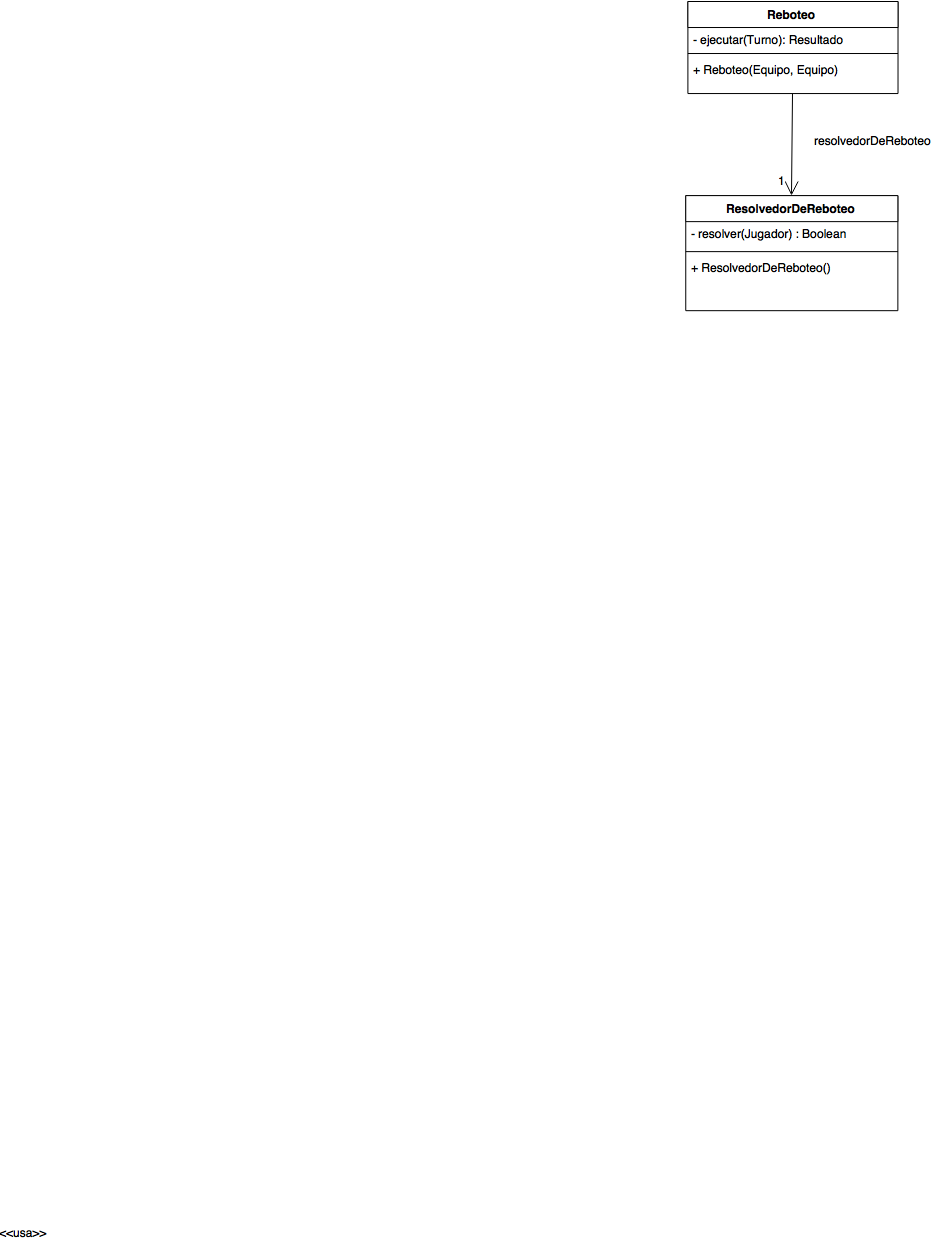
\includegraphics[scale=0.25]{imagenes/diagrama-clases-reboteo.png}
  \caption{Diagrama de clases para el movimiento de reboteo}
\end{figure}

A continuación, un diagrama de secuencia que representa la ejecución de un reboteo.

\begin{landscape}

  \begin{figure}[h!]
   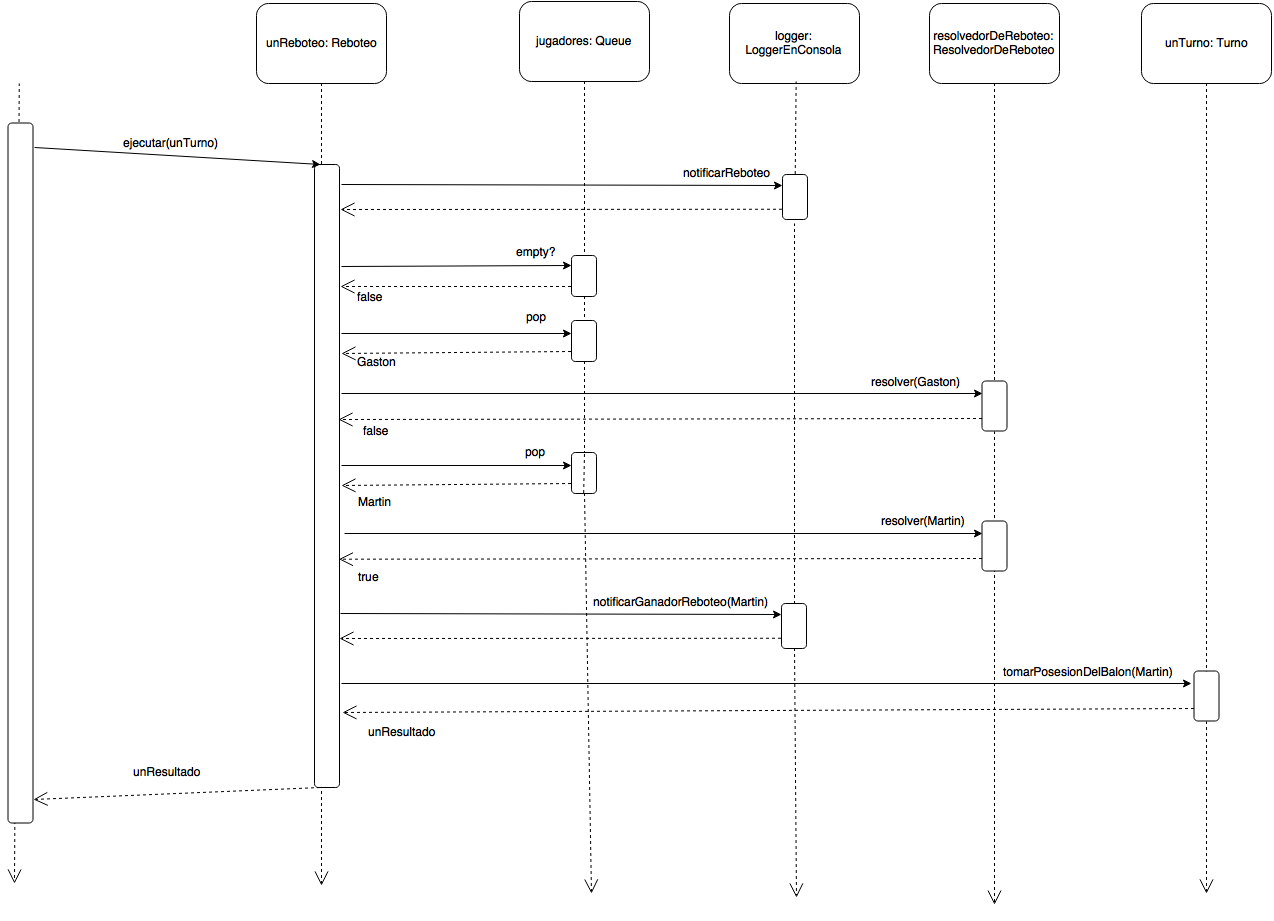
\includegraphics[scale=0.35]{imagenes/reboteo.png}
   \caption{Un reboteo cuyo ganador es Martin.}
  \end{figure}

\end{landscape}


